\subsection{Visualizzazione test salvati}

\begin{figure}[H]
    \centering
    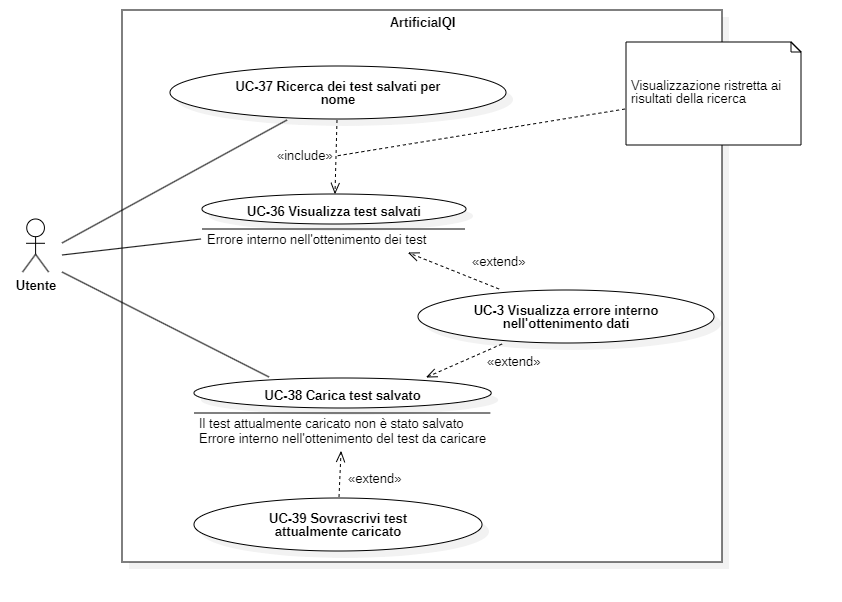
\includegraphics[scale=0.25]{Sezioni/UseCase/Immagini/VisualizzazioneTestSalvati}
    \caption{Diagramma per la visualizzazione di test salvati.}
\end{figure}

\begin{usecase}{UC-39}{Visualizza test salvati}
    \label{uc:UC-39}
    
    \req{\hyperref[ru:RUF-1]{RUF-1}}
    
    \pre{}
    
    \post{
        \item L'utente visualizza le esecuzioni di test salvate
    }
    
    \actor{
        Utente
    }
    
    \subactors{}
    
    \trigger{L'utente vuole visualizzare i test salvati}
    
    \inc{}
    
    \base{}
    
    \scenario{
        \item L'utente richiede la visualizzazione dei test salvati
        \item Il sistema ottiene i test salvati
        \item Il sistema visualizza i test salvati sotto forma di una lista
    }
    
    \subscenario{
        \item[2.1] Non esistono test salvati:
        \begin{itemize}
            \item Il sistema indica all'utente che non esistono test salvati
        \end{itemize}
        \item[2.2] Il sistema verifica un errore interno durante l'ottenimento dei test salvati:
        \begin{itemize}
            \item \hyperref[uc:UC-3]{UC-3}
        \end{itemize}
    }

\end{usecase}

\begin{usecase}{UC-40}{Ricerca dei test salvati per nome}
    \label{uc:UC-40}
    
    \req{\hyperref[ru:RUF-2]{RUF-2}}
    
    \pre{
        \item L'utente sta visualizzando i test salvati
    }
    
    \post{
        \item L'utente visualizza l'insieme di test salvati risultanti dalla ricerca
    }
    
    \actor{
        Utente
    }
    
    \subactors{}
    
    \trigger{L'utente vuole visualizzare i test salvati}
    
    \inc{\hyperref[uc:UC-39]{UC-39}}
    
    \base{}
    
    \scenario{
        \item L'utente indica le parole chiave da usare nella ricerca
        \item L'utente richiede l'esecuzione della ricerca
        \item Il sistema restringe i test salvati all'insieme di test che contengono nel proprio nome le parole chiave
        \item L'insieme di test ristretto viene visualizzato seguendo \hyperref[uc:UC-39]{UC-39}
    }
    
    \subscenario{}
\end{usecase}

\begin{usecase}{UC-41}{Carica test salvato}
    \label{uc:UC-41}
    
    \req{\hyperref[ru:RUF-3]{RUF-3}}
    
    \pre{
        \item L'utente sta visualizzando i test salvati
    }
    
    \post{
        \item Il test indicato dall'utente viene caricato nel sistema
    }
    
    \actor{
        Utente
    }
    
    \subactors{}
    
    \trigger{L'utente vuole caricare un test salvato}
    
    \inc{}
    
    \base{}
    
    \scenario{
        \item L'utente richiede il caricamento di un test visualizzato
        \item Il sistema verifica che il test attualmente caricato sia stato salvato
        \item Il sistema carica il test indicato
    }
    
    \subscenario{
        \item[2.1] Esiste un test attualmente caricato che non è stato salvato:
        \begin{itemize}
            \item \hyperref[uc:UC-42]{UC-42}
        \end{itemize}
        \item[2.2] Avviene un errore interno durante l'ottenimento del test indicato:
        \begin{itemize}
            \item \hyperref[uc:UC-3]{UC-3}
        \end{itemize}
    }
\end{usecase}

\begin{usecase}{UC-42}{Sovrascrivi test attualmente caricato}
    \label{uc:UC-42}
    
    \req{}
    
    \pre{
        \item Esiste un test caricato che non è ancora stato salvato
    }
    
    \post{
        \item Il test indicato dall'utente viene caricato nel sistema
    }
    
    \actor{Utente}
    
    \subactors{}
    
    \trigger{Il sistema deve caricare un test e quello attualmente caricato non è ancora stato salvato nel sistema}
    
    \inc{}
    
    \base{}
    
    \scenario{
        \item Il sistema richiede la conferma della sovrascrittura
        \item Il sistema procede con la sovrascrittura del test caricato che viene perso
    }
    
    \subscenario{
        \item[1.1] L'utente annulla la sovrascrittura:
        \begin{itemize}
            \item L'operazione di sovrascrittura termina
            \item Il test caricato resta invariato
        \end{itemize}
    }
\end{usecase}